\documentclass{sigplanconf}[10pt]

% TODO: explain that we have not observed overflows in the safe instructions.
% TODO: explain that u-SSA does not yield noticeable performance improvements.

\usepackage{amsmath}
\usepackage{graphicx}
\usepackage{mathpartir} % To use \inferrule
\usepackage{amssymb}    % To use \mathbb
\usepackage{skak}
\usepackage{pbox}

\newtheorem{definition}[section]{Definition}

% Definition of new commands that I use in this text:
\newcommand{\fun}[1]{\mbox{\textbf{#1}}}
\newcommand{\lb}[1]{#1_{\downarrow}}
\newcommand{\ub}[1]{#1_{\uparrow}}
\newcommand{\varset}[1]{\mbox{$\cal{#1}$}}
\newcommand{\code}[1]{\textbf{#1}}

\setlength{\textfloatsep}{12.0pt plus 1.0pt minus 1.0pt}


\begin{document}

\conferenceinfo{CGO '13}{February 23 - February 27. Shenzhen, China} 
\copyrightyear{2013}
\copyrightdata{[to be supplied]} 

\titlebanner{Code Generation and Optimization}        % These are ignored unless
\preprintfooter{Overflow Elimination}   % 'preprint' option specified.

\title{A fast and Low-Overhead Technique to Secure Programs Against
Integer Overflows}
%\subtitle{A case study of the Dinamica EGO toolkit}

\authorinfo{Raphael Ernani Rodrigues, Victor Hugo Sperle Campos,
Fernando Magno Quint\~{a}o Pereira}
           {Department of Computer Science -- The Federal University of Minas Gerais (UFMG) -- Brazil}
           {\{raphael,victorsc,fernando\}@dcc.ufmg.br}

\maketitle

\begin{abstract}
The integer primitive type has upper and lower bounds in many programming
languages, including C, and Java.
These limits might lead programs that manipulate large integer numbers to
produce unexpected results due to overflows.
There exists a plethora of works that instrument programs to track the occurrence
of these overflows.
In this paper we present an algorithm that uses static range analysis to
avoid this instrumentation whenever possible.
Our range analysis contains novel techniques, such as a notion of ``future"
bounds to handle comparisons between variables.
We have used this algorithm to avoid some checks created by a dynamic instrumentation
library that we have implemented in LLVM.
This framework has been used to detect overflows in hundreds of C/C++ programs.
As a testimony of its effectiveness, our range analysis has been able to avoid
25\% of all the overflow checks necessary to secure the C programs in the
LLVM test suite.
This optimization has reduced the runtime overhead of instrumentation by 50\%.
\end{abstract}

\category{D.3.4}{Processors}{Compilers}

\terms
Languages, Performance

\keywords
Integer Overflow, Compiler, Range analysis

\section{Introduction}
\label{sec:int}

% What are integer overflows.
The most popular programming languages, including C, C++ and Java, limit the
size of primitive numeric types.
For instance, the \texttt{int} type, in C++, ranges from $-2^{31}$ to
$2^{31}-1$.
Consequently, there exist numbers that cannot be represented by these types.
In general, these programming languages resort to a {\em wrapping-arithmetics}
semantics~\cite{Warren02} to perform integer operations.
If a number $n$ is too large to fit into a primitive data type $T$, then $n$'s
value wraps around, and we obtain $n \ \mbox{modulo} \ T_{max}$.
There are situations in which this semantics is acceptable~\cite{Dietz12}.
For instance, programmers might rely on this behavior to implement hash
functions and random number generators.
On the other hand, there exist also situations in which this behavior might
lead a program to produce unexpected results.
As an example, in 1996, the Ariane 5 rocket was lost due to an arithmetic
overflow -- a bug that resulted in a loss of more than US\$370 million~\cite{Dowson97}.

% TODO We need to explain better the wrapping-arithmetics, and we need to cite it
% properly. What could be a good (official) citation?


% Why there is still the need to devise efficient methods to eliminate them.
Programming languages such as Ada or Lisp can be customized to throw exceptions
whenever integer overflows are detected.
Furthermore, there exist recent works proposing to instrument binaries
derived from C, C++ and Java programs to detect the occurrence of overflows
dynamically~\cite{Brumley07,Dietz12}.
Thus, if an overflow happens, then the instrumented program can take some
action, such as to log the event, or to terminate the program.
However, this safety comes with a price: arithmetic operations need to be
surveilled, and the runtime checks cost time.
Zhang {\em et al.}~\cite{Zhang10} have proposed to eliminate some of this
overhead via a tainted flow analysis.
We have a similar goal, yet, our approach is substantially different.

% Our contribution: range analysis.
This paper describes the range analysis algorithm that
we have developed to eliminate overflow checks in instrumented programs.
As we show in Section~\ref{sec:range}, our algorithm has three core insights.
Firstly, in Section~\ref{sub:micro} we propose a three-phase approach to extract
information from comparisons between variables, e.g., $x < y$.
Previous algorithms either deal with these comparisons via
expensive relational analyses~\cite{Cousot78,Lakhdar11,Mine06}, or only
consider comparisons between variables and
constants~\cite{Mahlke01,Patterson95,Stephenson00}.
Secondly, in Section~\ref{sub:prop} we show how we rely on strongly connected
components to achieve speed and precision.
It is well-known that this technique is effective in speeding up constraint
resolution~\cite[Sec 6.3]{Nielson99}.
However, given our three-phase approach, we improve precision
by solving strong components in topological order.
Finally, in Section~\ref{sub:splitting} we propose a new program representation that
is more precise than other intermediate forms used to solve range
analysis sparsely.
This new live range splitting strategy is only valid if the instrumented
program terminates whenever an integer overflow is detected.
If we cannot rely on this guarantee, then our more conservative live range splitting
strategy produces the program representation that Bodik
{\em et al.}~\cite{Bodik00} call Extended Static Single Assignment
form.
In Section~\ref{sub:range} we show that an interprocedural implementation of our
algorithm analyzes programs with half-a-million lines of code in less than ten
seconds.
Furthermore, the speed and memory consumption of our range analysis grows linearly
with the program size.

% Our experimental results.
We use our range analysis to reduce the runtime overhead imposed by a dynamic
instrumentation library.
This instrumentation framework, a contribution of this paper that we describe in
Section~\ref{sec:dyn}, has been implemented in the LLVM compiler~\cite{Lattner04}.
We have logged overflows in a vast number of programs, and in this
paper we focus on SPEC CPU 2006.
We have re-discovered the integer overflows recently observed by
Dietz {\em et al.}~\cite{Dietz12}.
The performance of our instrumentation library, even without the support of range
analysis, is within the 5\% runtime overhead of Brumley {\em et al.}'s~\cite{Brumley07}
state-of-the-art algorithm.
The range analysis halves down this overhead.
Our static analysis algorithm avoids 24.93\% of the overflow
checks created by the dynamic instrumentation framework.
With this support, the instrumented SPEC programs are only 1.73\% slower.
Therefore, we show in this paper that securing programs against integer overflows
is very cheap.

\noindent
\textbf{The Danger that Integer Overflows Represent: }
Figure~\ref{fig:ex_buffer_overflow} illustrates an example of integer
overflow vulnerability.
This vulnerability allows an adversary to perform a buffer overrun attack
on a program that is apparently guarded against this type of exploit.
We will use the C datatype \texttt{char}, which represents
signed 8-bit numbers, so that the interested reader can easily
reconstruct this exploit.
Examples of actual vulnerabilities, with larger primitive types, are given
by Brumley {\em et al.}~\cite{Brumley07}, Dietz {\em et al.}~\cite{Dietz12},
and Zhang {\em et al.}~\cite{Zhang10}.
The function \texttt{read\_matrix} copies the linearized matrix \texttt{data}
into \texttt{buf}, to later process it, in line 12.
The arguments \texttt{w} and \texttt{h} determine the number of rows and
columns in the matrix.
If the \texttt{char} datatype could represent arbitrarily long numbers, then
this function would be safe against buffer overruns, due to the test at
line 3.
However, if, for instance, we have that \texttt{w}$= 6$ and \texttt{h}$= 22$,
then \texttt{buf\_size}$= -124$, due to the wrapping semantics of
integer arithmetics in C.
In this case, twelve words in the activation record of \texttt{read\_matrix}
would be overwritten.
By carefully crafting the contents of \texttt{data}, an adversary can, in this
way, change the return address of \texttt{read\_matrix}, diverting program's
execution to a system's function, such as \texttt{telnet}, for instance.

\begin{figure}[t!]
\begin{center}
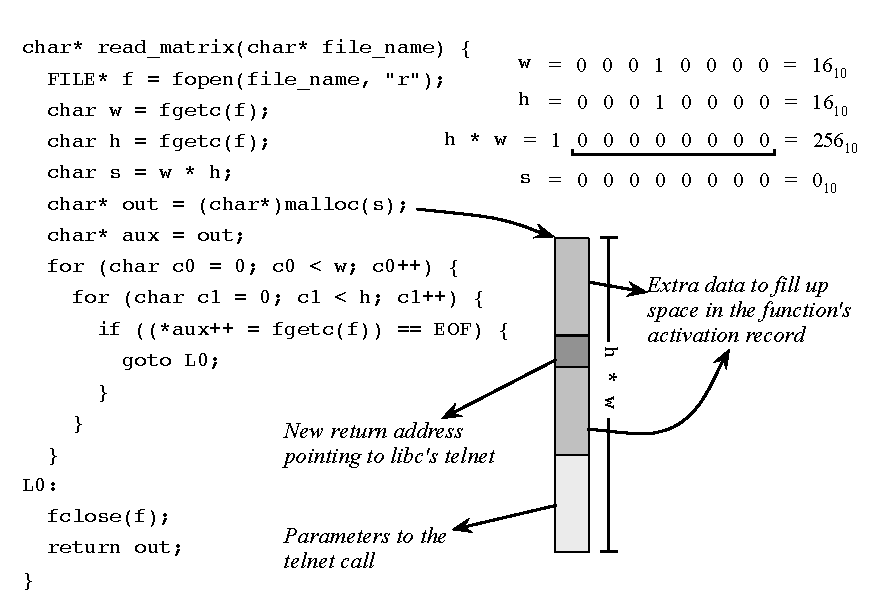
\includegraphics[width=\columnwidth]{images/ex_buffer_overflow}
\end{center}
\caption{\label{fig:ex_buffer_overflow}
An example of an exploitable integer overflow vulnerability.}
\end{figure}

\section{Range Analysis}
\label{sec:range}

\subsection{The Interval Lattice}
\label{sub:lattice}

% Define the lattice, the constraints and the valuation I.
Following Gawlitza {\em et al.}'s notation~\cite{Gawlitza09}, we shall be
performing arithmetic operations over the complete lattice
$\cal{Z} = \mathbb{Z} \cup \{-\infty, +\infty\}$, where the ordering is
naturally given by $-\infty < \ldots < -2 < -1 < 0 < 1 < 2 < \ldots +\infty$.
For any $x > -\infty$ we define:

\begin{tabular}{lcl}
$x + \infty = \infty$ & \mbox{\hspace{0.1cm}} & $x - \infty = - \infty, x \neq +\infty$ \\
$x \times \infty = \infty$ if $x > 0$ & & $x \times \infty = -\infty$ if $x < 0$ \\
$0 \times \infty = 0$ & & $(-\infty) \times \infty = \ $ not defined $$ \\
\end{tabular}

Notice that $(\infty -\infty)$ is not well-defined.
From the lattice $\varset{Z}$ we define the product lattice
$\varset{Z}^2$ as follows:
%
\begin{equation*}
\varset{Z}^2 = \{ \emptyset \} \cup \{[z_1, z_2] | \ z_1,z_2 \in \varset{Z},
\ z_1 \leq z_2, \  -\infty < z_2 \}
\end{equation*}
%
This interval lattice is partially ordered by the subset relation, which we
denote by ``$\sqsubseteq$".
Range intersection, ``$\sqcap$", is defined by:
\[
[a_1, a_2] \sqcap [b_1, b_2] =
\begin{cases}
[\mbox{max}(a_1, b_1), \mbox{min}(a_2, b_2)], \ \mbox{if} \ a_1 \leq b_1 \leq a_2  \\ \ \ \ \ \mbox{or} \ b_1 \leq a_1 \leq b_2 \\
[a_1, a_2] \sqcap [b_1, b_2] = \emptyset, \ \mbox{otherwise}
\end{cases}
\]
And range union, ``$\sqcup$", is given by:
\[
[a_1, a_2] \sqcup [b_1, b_2] = [\mbox{min}(a_1, b_1), \mbox{max}(a_2, b_2)]
\]

Given an interval $\iota = [l, u]$, we let $\lb{\iota} = l$, and
$\ub{\iota} = u$, where $\lb{\iota}$ is the lower bound and $\ub{\iota}$ is
the upper bound of a variable.
We let \varset{V} be a set of constraint variables, and
$I: \varset{V} \mapsto \varset{Z}^2$ a
mapping from these variables to intervals in $\varset{Z}^2$.
Our objective is to solve a constraint system \varset{C}, formed by constraints
such as those seen in Figure~\ref{fig:eval_function}(left).
We let the $\phi$-functions be as defined by Cytron
{\em et al.}~\cite{Cytron91}: they join different variable names into a single
definition.
Figure~\ref{fig:eval_function}(right) defines a valuation function $e$ on the
interval domain.
Armed with these concepts, we define the range analysis problem as follows: \\

\noindent
\textsc{Definition: Range Analysis Problem} \\
\textbf{Input:} a set \varset{C} of constraints ranging over a set
\varset{V} of variables. \\
\textbf{Output:} a mapping I such that, for any
$V \in \varset{V}$, e(V) = I[V].

\begin{figure}[t!]
\begin{center}
\begin{small}
\begin{eqnarray*}
\begin{array}{r@{\hspace{.5cm}}c}
Y = [l, u]
&
e(Y) = [l, u]
\\
\\
Y = \phi (X_1, X_2)
&
\inferrule{I[X_1]=[l_1, u_1] \\ I[X_2]=[l_2, u_2]}
{e(Y) = [l_1, u_1] \sqcup [l_2, u_2]}
\\
\\
Y = X_1 + X_2
&
\inferrule{I[X_1]=[l_1, u_1] \\ I[X_2]=[l_2, u_2]}
{e(Y) = [l_1 + l_2, u_1 + u_2]}
\\
\\
Y = X_1 \times X_2
&
\inferrule{L = \{l_1l_2, l_1u_2, u_1l_2, u_1u_2\} \\ I[X_1]=[l_1, u_1] \\ I[X_2]=[l_2, u_2]}
{e(Y) = [\mbox{min}(L), \mbox{max}(L)]}
\\
\\
Y = aX + b
&
\inferrule{I[X]=[l, u] \\ k_l = al + b \\ k_u = au + b}
{e(Y) = [\mbox{min}(k_l, k_u), \mbox{max}(k_l, k_u)]}
\\
\\
Y = X \sqcap [l', u']
&
\inferrule{I[X]=[l, u]}
{e(Y) \leftarrow [l, u] \sqcap [l', u']}
\end{array}
\end{eqnarray*}
\caption{\label{fig:eval_function}
A suite of constraints that produce an instance of the range analysis problem.}
\end{small}
\end{center}
\end{figure}

We will use the program in Figure~\ref{fig:ex_eSSA_cgo}(a) to illustrate our
range analysis.
Figure~\ref{fig:ex_eSSA_cgo}(b) shows the same program in e-SSA
form~\cite{Bodik00},
and Figure~\ref{fig:ex_eSSA_cgo}(c) outlines the constraints that we extract
from this program.
There is a clear correspondence between instructions and constraints.
Our analysis is sparse~\cite{Choi91}; thus, we associate one, and only one,
constraint with each integer variable defined in the program.
A possible solution to the range analysis problem, as obtained via the
techniques that we will introduce in Section~\ref{sub:prop}, is given in
Figure~\ref{fig:ex_eSSA_cgo}(d).

\begin{figure}[t!]
\begin{center}
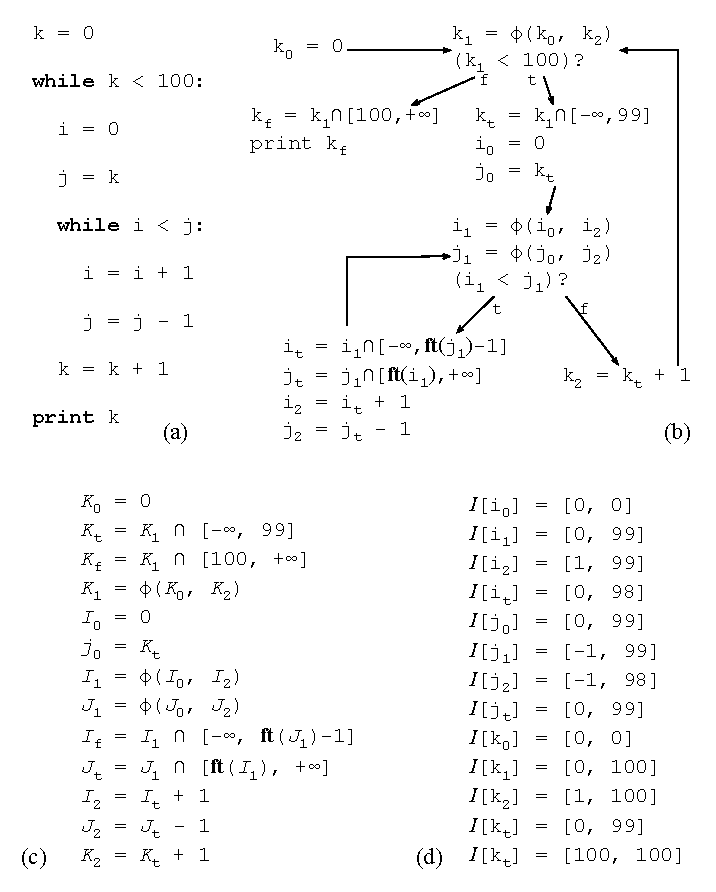
\includegraphics[width=\columnwidth]{images/ex_eSSA_cgo}
\end{center}
\caption{\label{fig:ex_eSSA_cgo}
(a) Example program.
(b) Control Flow Graph in e-SSA form.
(c) Constraints that we extract from the program.
(d) Possible solution to the range analysis problem.}
\end{figure}

\subsection{Range Propagation}
\label{sub:prop}

% The macro algorithm
Our range analysis algorithm works in a number of steps.
Firstly, we convert the program to an intermediate representation that gives
us subsidies to perform a sparse analysis.
We have tested our algorithm with two different representations, as we discuss
in Section~\ref{sub:splitting}.
Secondly, we extract constraints from the program representation.
Thirdly, we build a constraint graph, following the strategy pointed by
Su and Wagner~\cite{Su05}.
However, contrary to them, in a next phase we find the strongly connected
components in this graph, collapse them into super-nodes, and sort the
resulting digraph topologically.
Finally, for each strong component, we apply a three-phase approach to determine
the ranges of the variables.

\noindent
\textbf{Building the Constraint Graph. }
Given a set $\varset{C}$ of constraints, which define and/or use constraint
variables from a set $\varset{V}$, we build a constraint graph
$G = (\varset{C} \cup \varset{V}, E)$.
The vertices in \varset{C} are the {\em constraint nodes}, and the
nodes in \varset{V} are the {\em variable nodes}.
If $V \in \varset{V}$ is used in constraint $C \in \varset{C}$, then
we create an edge $\overrightarrow{VC}$.
If constraint $C \in \varset{C}$ defines variable $\varset{V} \in V$, then we
create an edge $\overrightarrow{CV}$.
Figure~\ref{fig:ex_graph} shows the constraint graph that we build for the
program in Figure~\ref{fig:ex_eSSA_cgo}(b).
Our algorithm introduces the notion of {\em future ranges}, which we use to extract
range information from comparisons between variables.
In Section~\ref{sub:splitting} we explain how futures are created.
If $V$ is used by constraint $C$ as the input of a future range, then the edge
from $V$ to $C$ represents what Ferrante {\em et al.} call a {\em control
dependence}~\cite[p.323]{Ferrante87}.
We use dashed lines to represent these edges.
All the other edges denote {\em data dependences}~\cite[p.322]{Ferrante87}.
As we will show later, control dependence edges increase the precision of our
algorithm to solve future bounds.

\begin{figure}[t!]
\begin{center}
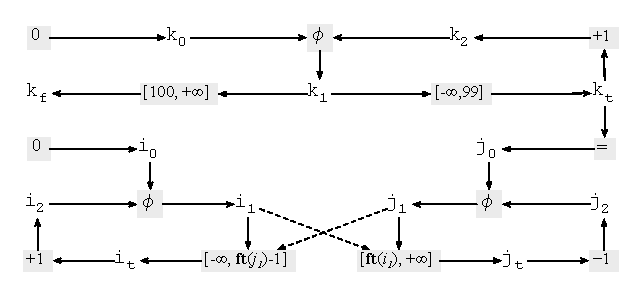
\includegraphics[width=\columnwidth]{images/ex_graph}
\end{center}
\caption{\label{fig:ex_graph}
The constraint graph that we build for the program in
Figure~\ref{fig:ex_eSSA_cgo}(b).}
\end{figure}

\noindent
\textbf{Propagating Ranges in Topological Order. }
After building the constraint graph, we find its strongly connected components.
We collapse these components in super nodes, and then propagate
ranges along the resulting digraph.
This approach is essential for scalability, because all the complexity of our
algorithm lies in the resolution of strong components.
Our tests show that the vast majority of the strongly connected components are
singletons.
For instance, 99.11\% of the SCCs in SPEC CPU 2006 dealII (\texttt{447.dealII}) have
only one node.
Moreover, the composite components usually contain a small number of nodes.
As an example, the largest component in dealII has 2,131 nodes,
even though dealII's constraint graph has over one million nodes.
This large SCC exists due to a long chain of mutually recursive function calls.

\subsection{A Three-Phase Approach to Solve Strong Components}
\label{sub:micro}

We find the ranges of the variables in each strongly connected component in
three phases.
First we determine the growth pattern of each variable in the component via
widening.
In the second step, we replace future bounds by actual limits.
Finally, a narrowing phase starting from conditional tests improves the
precision of our results.

\noindent
\textbf{Widening: } we start solving constraints by determining how each
program variable might grow.
For instance, if a variable is only updated by sums with positive numbers, then
it only grows up.
If, instead, a variable is only updated by sums with negative numbers, then it
grows down.
Some variables can also grow in both directions.
We discover these growth patterns by abstractly interpreting the constraints
that constitute the strongly connected component.
We ensure termination via a widening operator.
Our implementation uses {\em jump-set widening}, which is typically used in
range analysis~\cite[p.228]{Nielson99}.
This operator is a generalization of Cousot and Cousot's original widening
operator~\cite{Cousot77}, which we describe below:
%
\begin{equation*}
I[Y] =
\begin{cases}
\mbox{if} \ I[Y] = [\bot, \bot] \ \mbox{then} \ e(Y) \\
\mbox{elif} \ \lb{e(Y)} < \lb{I[Y]}  \ \mbox{and} \ \ub{e(Y)} > \ub{I[Y]} \ \mbox{then} \ [-\infty, \infty] \\
\mbox{elif} \ \lb{e(Y)} < \lb{I[Y]} \ \mbox{then} \ [-\infty, \ub{I[Y]}] \\
\mbox{elif} \ \ub{e(Y)} > \ub{I[Y]} \ \mbox{then} \ [\lb{I[Y]}, \infty]
\end{cases}
\end{equation*}
%
We let $\lb{[l, u]} = l$ and $\ub{[l, u]} = u$.
We let $\bot$ denote non-itialized intervals, so that $[\bot, \bot] \sqcup
[l, u] = [l, u]$.
This operation only happens at $\phi$-nodes, because we evaluate constraints in
topological order.
The map $I$ and the abstract evaluation function $e$ are determined as in
Figure~\ref{fig:eval_function}.
We have an implementation of $e$ for each operation that the
target programming language provides.
Our current LLVM implementation has 18 different instances of $e$, including
signed and unsigned addition, subtraction, multiplication and division, plus
truncation, the bitwise integer operators and $\phi$-functions.

If we use the widening operator above, then the abstract state of any constraint
variable can only change three times, e.g., $[\bot, \bot] \rightarrow [c_1, c_2]
\rightarrow [c_1, \infty] \rightarrow [-\infty, \infty]$, or
$[\bot, \bot] \rightarrow [c_1, c_2] \rightarrow [-\infty, c_2]
\rightarrow [-\infty, \infty]$.
Therefore, we determine the growth behavior of each constraint variable in
a strong component in linear time on the number of constraints in that
component.
Figure~\ref{fig:ex_partition_grow_crop}(b) shows the abstract state of the
variables in the largest SCC of the graph in Figure~\ref{fig:ex_graph}.
As we see in the figure, this step of our algorithm has been able to determine
that variables \texttt{i}$_1$, \texttt{i}$_2$ and \texttt{i}$_t$ can only
increase, and that variables \texttt{j}$_1$, \texttt{j}$_2$ and \texttt{j}$_t$
can only decrease.

\begin{figure}[t!]
\begin{center}
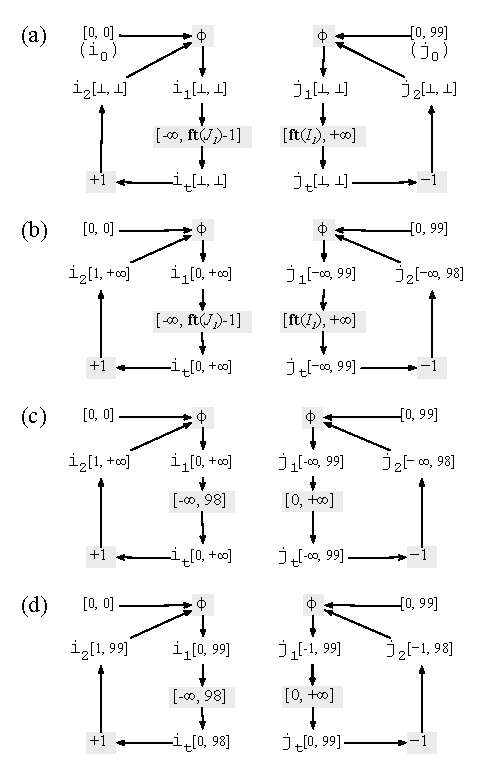
\includegraphics[width=0.9\columnwidth]{images/ex_partition_grow_crop}
\end{center}
\caption{\label{fig:ex_partition_grow_crop}
Four snapshots of the last SCC of Figure~\ref{fig:ex_graph}.
(a) After removing control dependence edges.
(b) After running the growth analysis.
(c) After fixing the intersections bound to futures.
(d) After running the narrowing analysis.}
\end{figure}

\noindent
\textbf{Future resolution: }
the next phase of the algorithm to determine intervals inside a strong
component consists in replacing futures by actual bounds, a task that we
accomplish by using the rules below:
%
\begin{eqnarray*}
\begin{array}{c}
\inferrule{Y = X \sqcap [l, \fun{ft}(V) + c] \\ \ub{I[V]} = u}
{Y = X \sqcap [l, u + c]} \mbox{\hspace{0.3cm}} u, c \in \mathbb{Z} \cup \{-\infty, \infty\}
\\
\\
\inferrule{Y = X \sqcap [\fun{ft}(V) + c, u] \\ \lb{I[V]} = l}
{Y = X \sqcap [l + c, u]} \mbox{\hspace{0.3cm}} l, c \in \mathbb{Z} \cup \{-\infty, \infty\}
\end{array}
\end{eqnarray*}
%
To correctly replace a future $\fun{ft}(V)$ that limits a constraint
variable $V'$, we need to have already applied the growth analysis onto $V$.
Had we considered only data dependence edges, then it would be possible
that $V'$'s strong component would be analyzed before $V$'s.
However, because of control dependence edges, this case cannot happen.
The control dependence edges ensure that any topological ordering of the
constraint graph either places $V$ before $V'$, or places these nodes
in the same strongly connected component.
For instance, in Figure~\ref{fig:ex_graph}, variables $j_1$ and $i_t$ are in
the same SCC only because of the control dependence edges.
Figure~\ref{fig:ex_partition_grow_crop}(c) shows the result of resolving
futures in our running example.
The information that we acquire from the growth analysis is essential in this
phase.
For instance, the growth analysis has found out that the value stored in
variable \texttt{i}$_1$ can only increase.
Given that this variable is assigned the initial value zero, we can replace
$\fun{ft}(I_1)$ with this value.

\noindent
\textbf{Narrowing: } the last step that we apply on the strongly connected
component is the narrowing phase.
In this step we use values extracted from conditional tests to restrict the
bounds of the constraint variables.
We use the narrowing operator firstly proposed by Cousot and
Cousot~\cite{Cousot77}, which we show below:
%
\begin{equation*}
I[Y] =
\begin{cases}
\mbox{if} \ \lb{I[Y]} = -\infty  \ \mbox{and} \ \lb{e(Y)} > -\infty \ \mbox{then} \ [\lb{e(Y)}, \ub{I[Y]}] \\
\mbox{elif} \ \ub{I[Y]} = \infty \ \mbox{and} \ \ub{e(Y)} < \infty \ \mbox{then}
\ [\lb{I[Y]}, \ub{e(Y)}] \\
\mbox{elif} \ \lb{I[Y]} > \lb{e(Y)} \ \mbox{then} \ [\lb{e(Y)}, \ub{I[Y]}] \\
\mbox{elif} \ \ub{I[Y]} < \ub{e(Y)} \ \mbox{then} \ [\lb{I[Y]}, \ub{e(Y)}]
\end{cases}
\end{equation*}
%
Figure~\ref{fig:ex_partition_grow_crop}(d) shows the result of our narrowing
operator in our running example.
Ranges improve due to the two conditional tests in the program.
Firstly, we have that $I[I_t] = I[I_1] \sqcap [-\infty, 98]$, which gives us
that $I[I_t] = [0, 98]$.
We also have that $I[J_t] = I[J_1] \sqcap [0, \infty]$, giving
$I[J_t] = [0, 99]$.
From these new intervals, we can narrow the ranges bound to the other constraint
variables.

The combination of widening, futures and narrowing, plus use of strong components
gives us, in this example, a very precise solution.
We emphasize that finding this tight solution was only possible because of
the topological ordering of the constraint graph in Figure~\ref{fig:ex_graph}.
Upon meeting the constraint graph's last SCC, shown in
Figure~\ref{fig:ex_partition_grow_crop}, we had already determined that the
interval $[0, 0]$ is bound to $i_0$ and that the interval $[0, 99]$ is bound to
$j_0$, as we show in Figure~\ref{fig:ex_partition_grow_crop}(a).
Had we applied the widening operator onto the whole graph, then we would
have found out that variable $j_1$ is bound to $[-\infty, +\infty]$.
This imprecision happens because, on one hand $j_1$'s interval is influenced
by $k_t$'s, which is upper bounded by $+\infty$.
On the other hand $j_1$ is part of a decreasing cycle of dependences formed by
variables $j_t$ and $j_2$ in addition to itself.
Therefore, if we had applied the widening phase over the entire program followed
by a global narrowing phase, then we would not be able to recover some of
widening's precision loss.
However, because in this example we only analyze $j$'s SCC after we have
analyzed $k$'s, $k$ only contribute the constant range $[0, 99]$ to $j_0$.


\subsection{Live Range Splitting Strategies}
\label{sub:splitting}

A dense dataflow analysis associates information, i.e., a point in a lattice,
with each pair formed by a variable plus a program point.
If this information is invariant along every program point where the variable
is alive, then we can associate the information with the variable itself.
In this case, we say that the dataflow analysis is {\em sparse}~\cite{Choi91}.
A dense dataflow analysis can be transformed into a sparse one via a suitable
intermediate representation.
A compiler builds this intermediate representation by splitting the live ranges
of variables at the program points where the information associated with these
variables might change.
To split the live range of a variable $v$, at a program point $p$, we insert
a copy $v' = v$ at $p$, and rename every use of $v$ that is dominated by $p$.
In this paper we have experimented with two different live range splitting
alternatives.

The first strategy is the {\em Extended Static Single Assignment} (e-SSA) form,
proposed by Bodik {\em et al.}~\cite{Bodik00}.
We build the e-SSA representation by splitting live ranges at definition sites
-- hence it subsumes the SSA form -- and at conditional tests.
The program in Figure~\ref{fig:ex_eSSA_cgo}(b) is in e-SSA form.
Let $(v < c)?$ be a conditional test, and let $l_t$ and $l_f$ be labels in
the program, such that $l_t$ is the target of the test if the condition is true,
and $l_f$ is the target when the condition is false.
We split the live range of $v$ at any of these points if at least one of two
conditions is true:
(i) $l_f$ or $l_t$ dominate any use of $v$;
(ii) there exists a use of $v$ at the dominance frontier of $l_f$ or $l_t$.
For the notions of dominance and dominance-frontier, see Aho
{\em et al.}~\cite[p.656]{Aho06}.
To split the live range of $v$ at $l_f$ we insert at this
program point a copy $v_f = v \sqcap [c, +\infty]$, where $v_f$ is a fresh name.
We then rename every use of $v$ that is dominated by $l_f$ to $v_f$.
Dually, if we must split at $l_t$, then we create at this point a copy
$v_t = v \sqcap [-\infty, c-1]$, and rename variables accordingly.
If the conditional uses two variables, e.g., $(v_1 < v_2)?$, then we create
intersections bound to {\em futures}.
We insert, at $l_f$, $v_{1f} = v_1 \sqcap [\fun{ft}(v_2), +\infty]$,
and $v_{2f} = v_2 \sqcap [-\infty, \fun{ft}(v_1)]$.
Similarly, at $l_t$ we insert
$v_{1v} = v_1 \sqcap [-\infty, \fun{ft}(v_2) - 1]$
and $v_{2v} = v_2 \sqcap [\fun{ft}(v_1) + 1, +\infty]$.
A variable $v$ can never be associated with a future bound to
itself, e.g., $\fun{ft}(v)$.
This invariant holds because whenever the e-SSA conversion associates a variable
$u$ with $\fun{ft}(v)$, then $u$ is a fresh name created to split the live range
of $v$.

The second intermediate representation consists in splitting live ranges at
(i) definition sites -- it subsumes SSA, (ii) at conditional tests -- it
subsumes e-SSA, and at some use sites.
This representation, which we henceforth call u-SSA, is only valid if we
assume that integer overflows cannot happen.
We can provide this guarantee by using our dynamic instrumentation to terminate
a program in face of an overflow.
The rationale behind u-SSA is as follows: we know that past an instruction such
as $v = u + c, c \in \mathbb{Z}$ at a program point $p$, variable $u$ must be
less than $\mathit{MaxInt} - c$.
If that were not the case, then an overflow would have happened and the
program would have terminated.
Therefore, we split the live range of $u$ past its use point $p$, producing the
sequence $v = u + c; u' = u$, and renaming every use of $u$ that is dominated
by $p$ to $u'$.
We then associate $u'$ with the constraint $I[U'] \sqsubseteq I[U] \sqcap [-\infty, \mathit{MaxInt} - c]$.

\begin{figure}[t!]
\begin{center}
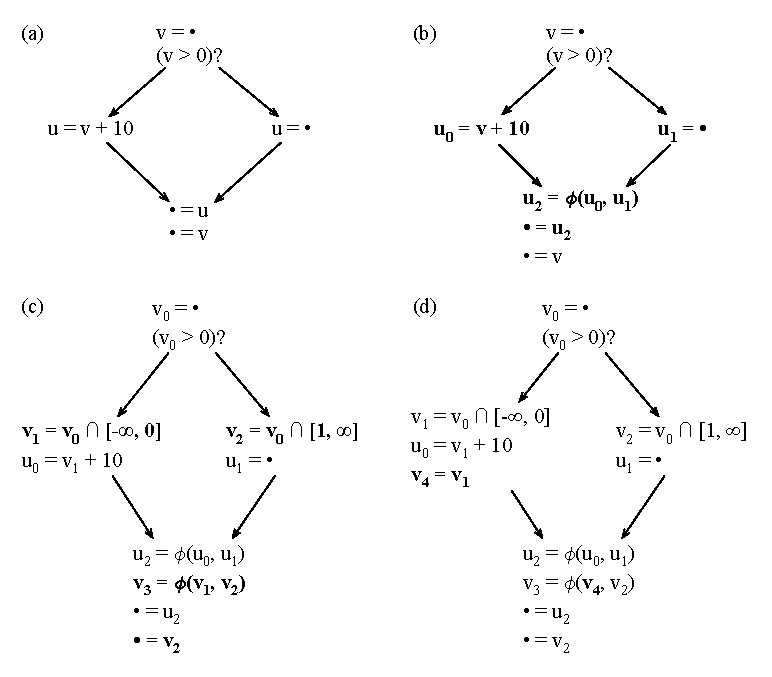
\includegraphics[width=\columnwidth]{images/ex_ir}
\end{center}
\caption{\label{fig:ex_ir}
(a) Example program.
(b) SSA form~\cite{Cytron91}.
(c) e-SSA form~\cite{Bodik00}.
(d) u-SSA form.}
\end{figure}

Figure~\ref{fig:ex_ir} compares the u-SSA form with the SSA and e-SSA
intermediate program representations.
We use the notation $v = \bullet$ to denote a definition of variable $v$, and
$\bullet = v$ to denote a use of it.
Figure~\ref{fig:ex_ir}(b) shows the example program converted to the SSA format.
Different definitions of variable $u$ have been renamed, and a
$\phi$-function joins these definitions into a single name.
The SSA form sparsifies a dataflow analysis that only extracts information from
the definition sites of variables, such as constant propagation.
Figure~\ref{fig:ex_ir}(c) shows the same program in e-SSA form.
This time we have renamed variable $v$ right after the conditional test where
this variable is used.
The e-SSA form serves dataflow analyses that acquire information from definition
sites and conditional tests.
Examples of these analyses include array bounds checking
elimination~\cite{Bodik00} and traditional implementations of range
analyses~\cite{Gough94,Patterson95}.
Finally, Figure~\ref{fig:ex_ir}(d) shows our example in u-SSA form.
The live range of variable $v_1$ has been divided right after its use.
This representation assists analyses that learn information from the way
that variables are used, and propagate this information forwardly.

\section{The Dynamic Instrumentation Library}
\label{sec:dyn}

%What is our instrumentation library
We have implemented our instrumentation library as a LLVM transformation pass;
thus, we work at the level of the compiler's intermediate
representation~\footnote{\texttt{http://llvm.org/docs/LangRef.html}}.
This is in contrast to previous work, which either transforms the
source code~\cite{Dietz12}, or the machine dependent code~\cite{Brumley07}.
We work at the intermediate representation level to be able to couple our
library with static analyses, such as the algorithm that we described in
Section~\ref{sec:range}.
Our instrumentation works by identifying the instructions that may 
lead to an overflow, and inserting assertions after those instructions. 
The LLVM IR has five instructions that may lead to an overflow:
\textsc{Add}, \textsc{Sub}, \textsc{Mul},  \textsc{Trunc} (also bit-casts) and
\textsc{Shl} (left shift).
Figure~\ref{fig:instrumentation} shows the dynamic tests that we perform to
detect overflows.

\begin{figure}[t!]
\begin{center}
\begin{tabular}{ll}
Instruction & Dynamic Check \\ \\
$x = o_1 \ +_s \ o_2$ & $(o_1 > 0 \wedge o_2 > 0 \wedge x < 0) \ \ \vee$ \\
                      & $(o_1 < 0 \wedge o_2 < 0 \wedge x > 0)$ \\ \\
$x = o_1 \ +_u \ o_2$ & $x < o_1 \vee x < o_2$ \\ \\
$x = o_1 \ -_s \ o_2$ & $(o_1 < 0 \vee o_2 > 0 \vee x > 0) \ \ \vee$ \\
                      & $(o_1 > 0 \vee o_2 < 0 \vee x < 0)$ \\ \\
$x = o_1 \ -_u \ o_2$ & $o_1 < o_2$ \\ \\
$x = o_1 \ \times_{u/s} \ o_2$ & $x \neq 0 \Rightarrow x \div o_1 \neq o_2$ \\ \\
$x = o_1 \ \qside \ n$ & $(o_1 > 0 \wedge x < o_1) \vee (o_1 < 0 \wedge n \neq 0)$ \\ \\
$x = \ \downarrow_n \ o_1$ & $\mbox{cast}(x, \mbox{type}(o_1)) \neq o_1$ \\ \\
$x = \ (\mbox{type}_n) o_1$ & $\mbox{cast}(x, \mbox{type}(o_1)) \neq o_1$ \\
\end{tabular}
\end{center}
\caption{\label{fig:instrumentation}Overflow checks. We use $\downarrow_n$ for
the operation that truncates to $n$ bits, and we use $(\mbox{type}_n)$ for a
bit-cast to $n$ bits. Both operations have the same semantics in our setting.
The subscript $s$ indicates a signed instruction; the subscript $u$ indicate
an unsigned operation.}
\end{figure}

%SUB instrumentation
The instrumentation that we insert is mostly straightforward.
We discuss in the rest of this section a few interesting cases.
When dealing with an unsigned \textsc{Sub} instruction, e.g,
$x = o_1 \ -_u \ o_2$, then a single check is enough to detect the bad
behavior: $o_1 < o_2$.
If $o_2$ is greater than $o_1$, then we assume that it is
a bug to try to represent a negative number in unsigned arithmetics.
Regarding multiplication, e.g., $x = o_1 \times o_2$, if $o_1 = 0$, then this
operation can never cause an overflow.
This test is necessary, because we check integer overflows in
multiplication via the inverse operation, e.g., integer division.
Thus, the test prevents a division by zero from happening.
The \textsc{Trunc} instruction, e.g., $x = \ \downarrow_n \ o_1$ assigns to $x$
the $n$ least significant bits of $o_1$.
The dynamic check, in this case, consists in expanding $x$ to
the datatype of $o_1$ and comparing the expanded value with $o_1$.
The LLVM IR provides instructions to perform these type expansions.
Note that our instrumentation catches any truncation that might result in
data loss, even if this loss is benign.
To make the dynamic checks more liberal, we give users the possibility of
disabling tests over truncations.

\paragraph{Practical Considerations. }
%Overview about the instrumentation technique
Our instrumentation library inserts new instructions into
the target program.
Although the dynamic check depends on the instruction that is instrumented,
the general modus operandi is the same.
Dynamic tests check for overflows after they happen.
The code that we insert to detect the overflow diverts the program flow in case
such an event takes place.
Figure~\ref{fig:instrumented_cfg} shows an actual control flow graph, before
and after the instrumentation.
Clearly the instrumented program will be larger than the original code.
Figure~\ref{fig:num_instructions} shows how many LLVM instructions are
necessary to instrument each arithmetic operation.
These numbers do not include the instructions necessary to handle the overflow
itself, e.g., block \texttt{\%11} in Figure~\ref{fig:instrumented_cfg}, as this
code is not in the program's main path.
Nevertheless, as we show empirically, this growth is small when
compared to the total size of our benchmarks, because most of the instructions
in these programs do not demand instrumentation.
Furthermore, none of the instructions used to instrument integer arithmetics
access memory.
Therefore, the overall slowdown that the instrumentation causes is usually
small, and the experiments in Section~\ref{sub:inst} confirm this
observation.

\begin{figure}[t!]
\begin{center}
\begin{small}
\renewcommand{\arraystretch}{1.5}
\begin{tabular}{lccccc}
& \textsc{Add} & \textsc{Sub} & \textsc{Mul} & \textsc{Shl} & \textsc{Trunc} \\
signed   & 12 & 12 & 6 & 8 & 3 \\
unsigned & 4  & 2  & 6 & 2 & 3
\end{tabular}
\end{small}
\caption{\label{fig:num_instructions}
Number of instructions used in each dynamic check.}
\end{center}
\end{figure}

\begin{figure}[t!]
\begin{center}
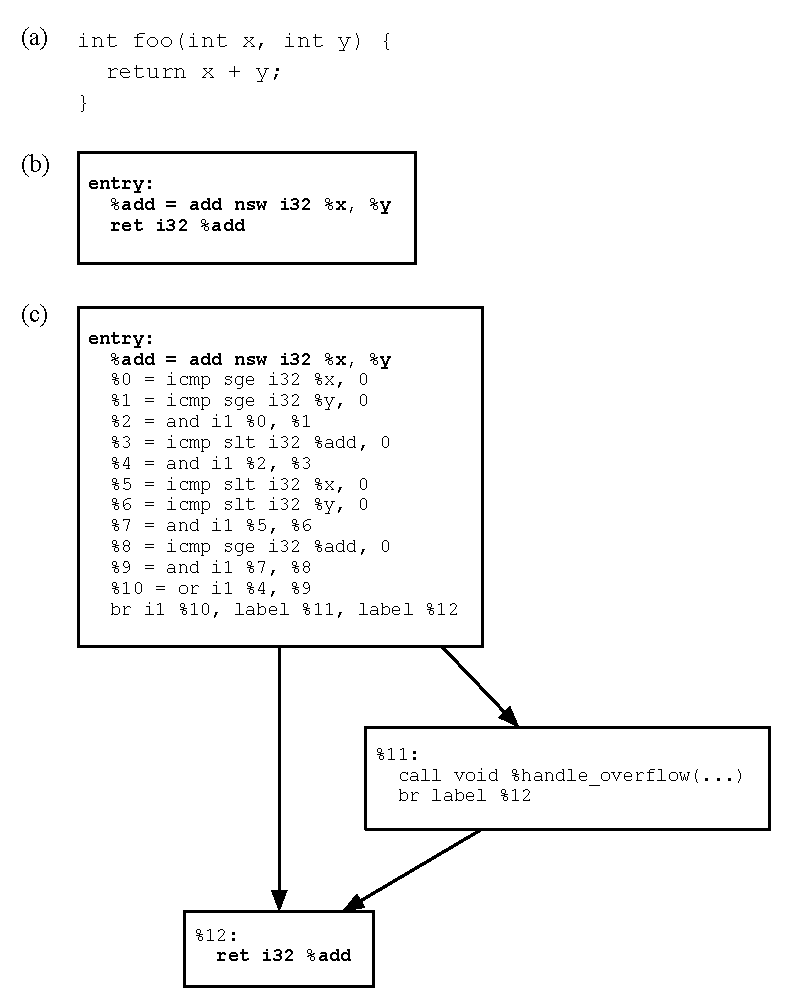
\includegraphics[width=\columnwidth]{images/instrumented_cfg}
\end{center}
\caption{\label{fig:instrumented_cfg}
(a) A simple C function.
(b) The same function converted to the LLVM intermediate representation.
(c) The instrumented code. The boldface lines were part of the original
program.}
\end{figure}

Which actions are performed once the overflow is detected depends on the
user, who has the option to overwrite the \texttt{handle\_ overflow}
function in Figure~\ref{fig:instrumented_cfg}.
Our library gives the user three options to handle overflows. 
First option: no-op.
This option allows us to verify the slowdown produced by the new instructions.
Second option: logging.
This is the standard option, and it preserves the behavior of the instrumented
program.
Whenever an overflow is detected, we print \texttt{Overflow detected in
FileName.cpp, line X.} in the standard error stream.
Third option: abort.
This option terminates the program once an overflow is detected.
Thus, it disallows undefined behavior due to integer overflows, and gives us the
opportunity to use the u-SSA form to get extra precision.

\paragraph{Using the static analysis to avoid some overflow checks.}
Our library can, optionally, use the range analysis to avoid having to
insert some overflow checks into the instrumented program.
We give the user the possibility of calling the range analysis with either the
e-SSA or the u-SSA live range splitting strategies.
Our static analysis classifies variables into four categories, depending on
their bounds:
\begin{itemize}
\item \textbf{Safe}: a variable is safe if its bounds are fully contained
inside its declared type.
For instance, if $x$ is declared as an unsigned 8-bits integer, then $x$ is
safe if its bounds are within the interval $[0, 255]$.
\item \textbf{Suspicious}: we say that a variable is suspicious if its bounds
go beyond the interval of its declared type, but the intersection between
these two ranges is non-empty.
For instance, the same variable $x$ would be suspicious if
$I[x] = [0, 257]$, as $\ub{I[x]} > \ub{\mathtt{uint8}}$.
\item \textbf{Uncertain}: we classify a variable as uncertain if at least one
of its limits is unbounded.
Our variable $x$ would be uncertain if $I[x] = [0, \infty]$.
We distinguish suspicious from uncertain variables because we speculate that
actual overflows are more common among elements in the former category.
\item \textbf{Buggy}: a variable is buggy if the intersection between its
inferred range and the range of its declared type is empty.
This is a definitive case of an overflow.
Continuing with our example, $x$ would be buggy if, for instance,
$I[x] = [257, \infty]$, given that $[257, \infty] \sqcap [0, 255] = \emptyset$.
\end{itemize}
Independent on the arithmetic instruction that is being analyzed, the
instrumentation library performs the same test:
if the result $x$ of an arithmetic instruction such as $x = o_1 +_s \ o_2$ is
safe, then the overflow check is not necessary, otherwise it must be
created.

\section{Experimental Results}
\label{sec:exp}

We have implemented our range analysis algorithm in LLVM 3.0, and have run
experiments on a Intel quad core CPU with a 2.40GHz clock, and 3.6GB of RAM.
Each core has a 4,096KB L1 cache.
We have used Linux Ubuntu 10.04.4.
Our implementation of range analysis has 3,958 lines of
commented C++ code, our e/u-SSA conversion module has 672 lines, and our
instrumentation pass has 762 lines.
We have analyzed 428 C programs that constitute the LLVM test suite plus the
integer benchmarks in SPEC CPU 2006.
Together, these programs contain 4.76 million assembly instructions.
This section has two main goals.
First, we want to show that our range analysis is fast and precise.
Second, we want to demonstrate the effectiveness of our framework to detect
integer overflows.

\subsection{Static Range Analysis}
\label{sub:range}

\noindent
\textbf{Time and Memory Complexity: }
Figure~\ref{fig:TimeCorr} compares the time to run our range analysis with the size of
the input programs.
We show data for the 100 largest benchmarks in our test suite, considering the number
of variable nodes in the constraint graph.
We perform function inlining before running our analysis.
Each point in the X line corresponds to a benchmark.
We analyze the smallest benchmark in this set, \texttt{Prolangs-C/deriv2}, which
has 1,131 variable nodes in the constraint graph, in 20ms.
We take 9.91 sec to analyze our largest benchmark, \texttt{403.gcc}, which,
after function inlining, has 1,419,456 assembly instructions, and a
constraint graph with 679,652 variable nodes.
For this data set, the coefficient of determination $(R^2)$ is 0.967, which
provides very strong evidence about the linear asymptotic complexity of our
implementation.

\begin{figure}[t!]
\begin{center}
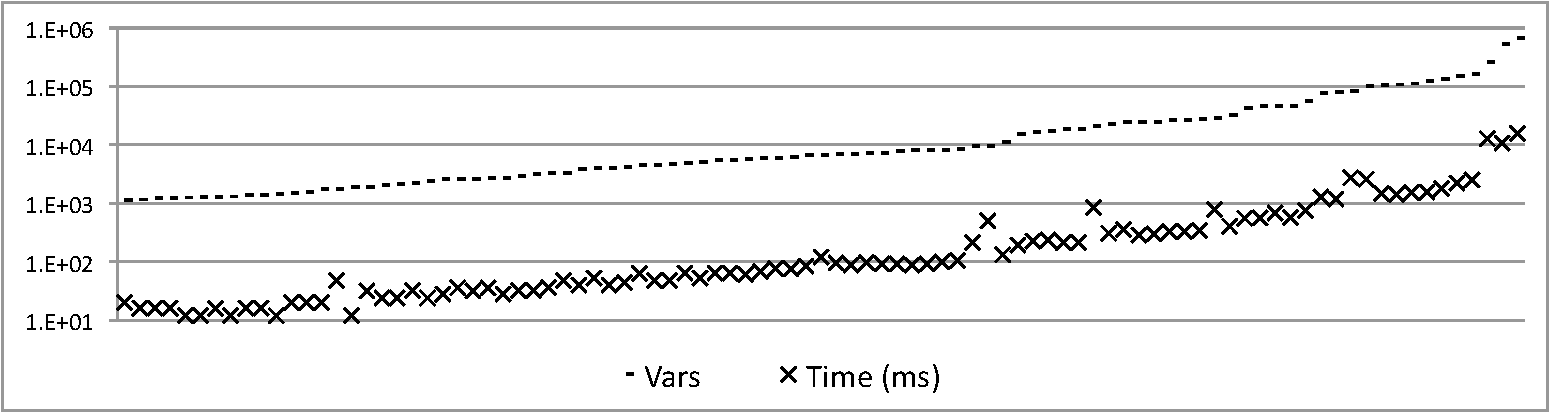
\includegraphics[width=\columnwidth]{images/TimeCorr}
\end{center}
\caption{\label{fig:TimeCorr}
Correlation between program size (number of var nodes in constraint
graphs) and analysis runtime (ms).
Each point represents a benchmark.
Coefficient of determination = 0.967.
}
\end{figure}

The experiments also reveal that the memory consumption of our implementation
grows linearly with the program size.
Figure~\ref{fig:MemCorr} plots these two quantities.
The linear correlation, in this case, is even stronger than that found in
Figure~\ref{fig:TimeCorr}: the coefficient of determination is 0.9947.
The figure only shows our 100 largest benchmarks.
Again, SPEC \texttt{403.gcc} is the largest benchmark, requiring
265,588KB to run.
Memory includes stack, heap and the executable program code.

\begin{figure}[t!]
\begin{center}
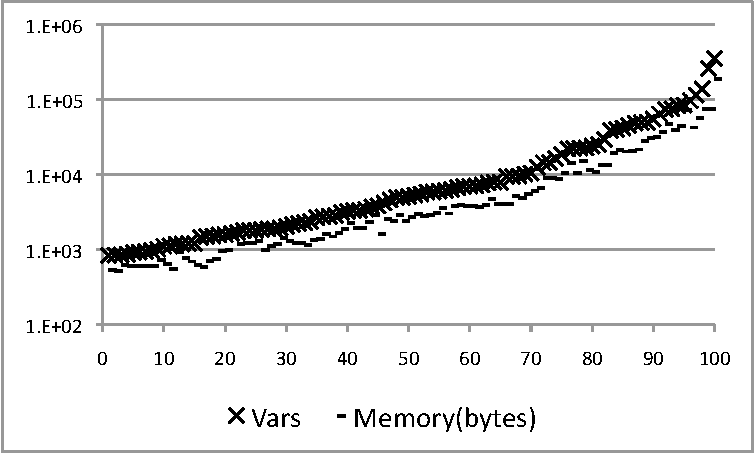
\includegraphics[width=\columnwidth]{images/MemCorr}
\end{center}
\caption{\label{fig:MemCorr}
Comparison between program size (number of var nodes in constraint
graphs) and memory consumption (KB).
Coefficient of determination = 0.9947.
}
\end{figure}

\noindent
\textbf{Precision: }
Our implementation of range analysis offers a good tradeoff between
precision and runtime.
Lakhdar {\em et al.}'s relational analysis~\cite{Lakhdar11}, for instance,
takes about 25 minutes to go over a program with almost 900 basic blocks.
We analyze programs of similar size in less than one second.
We do not claim our approach is as precise as such algorithms, even though we
are able to find exact bounds to 4/5 of the examples presented
in~\cite{Lakhdar11}.
On the contrary, we present a compromise between precision and speed
that scales to very large programs.
Nevertheless, our results are not trivial.
We have implemented a dynamic profiler that measures, for each variable,
its upper and lower limits, given an execution of the target program.
Figure~\ref{fig:precision} compares our results with those measured
dynamically for the Stanford benchmark, which is publicly
available in the LLVM test suite.
We chose Stanford because these benchmarks do not read data from external
files; hence, imprecisions are due exclusively to library functions that we cannot
analyze.

\begin{figure}[t!]
\begin{center}
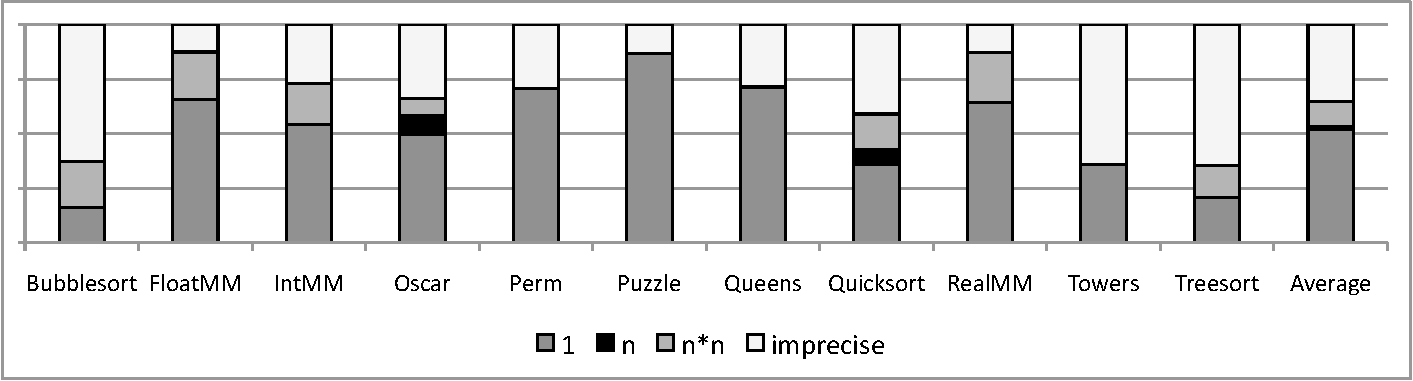
\includegraphics[width=\columnwidth]{images/precUpperBound}
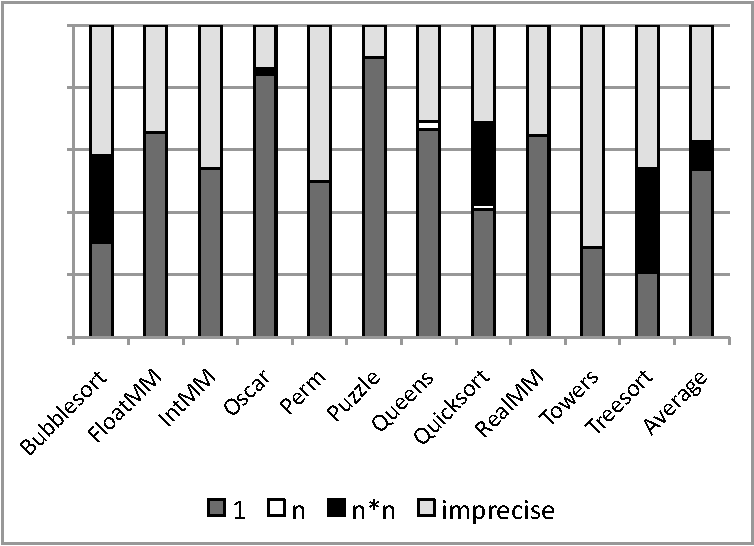
\includegraphics[width=\columnwidth]{images/precLowerBound}
\end{center}
\caption{\label{fig:precision}
(Upper) Comparison between static range analysis and dynamic profiler for
upper bounds.
(Lower) Comparison between static range analysis and dynamic profiler for
lower bounds.}
\end{figure}

We have classified the bounds estimated by the static analysis into four
categories.
The first category, called $1$, contains tight bounds:
during program execution, the variable has been assigned an upper,
or lower limit, that equals the limit inferred statically.
The second category, called $n$, contains the bounds that are
within twice the value inferred statically.
For instance, if the range analysis estimates that a variable $v$ is in the
range $[0, 100]$, and during the execution the dynamic profiler finds that
its maximum value is $51$, then $v$ falls into this category.
The third category, $n^2$, contains variables whose actual value is within
a quadratic factor of the estimated value.
In our example, $v$'s upper bound would have to be at most $10$ for it to
be in this category.
Finally, the fourth category contains variables whose estimated value lays
outside a quadratic factor of the actual value.
We call this category {\em imprecise}, and it contains mostly the limits that
our static analysis has marked as either $+\infty$ or $-\infty$.
As we see in Figure~\ref{fig:precision}, 54.11\% of the lower limits that
we have estimated statically are exact.
Similarly, 51.99\% of our upper bounds are also tight.
The figure also shows that, on average, 37.39\% of our lower limits are
imprecise, and 35.40\% of our upper limits are imprecise.
This result is on par with those obtained by more costly analysis, such as
Stephenson {\em et al.}'s~\cite{Stephenson00}.



%%%%%%%%%%%%%%%%%%%%%%%%%%%%%%%%%%%%%%%%%%%%%%%%%%%%%%%%%%%%%%%%%%%%%%%%%%%%%%%%%%
%Static Analysis
%%%%%%%%%%%%%%%%%%%%%%%%%%%%%%%%%%%%%%%%%%%%%%%%%%%%%%%%%%%%%%%%%%%%%%%%%%%%%%%%%%

%How we have done the dynamic tests
\subsection{The Instrumentation Library}
\label{sub:inst}

We have executed the instrumented programs of the integer benchmarks of SPEC
2006 CPU to probe the overhead imposed by our instrumentation.
These programs have been executed with their ``test" input sets.
We have not been able to run the binary that LLVM produces for SPEC's
\texttt{gcc} in our environment, even without any of our transformations, due
to an incompatible \texttt{ctype.h} header.
In addition, we have not been able to collect the statistics about
the overflows that occurred in SPEC's \texttt{bzip2}, because the log file
was too large.
We verified more than 3,000,000,000  overflows in this program.
Figure~\ref{fig:unprunedTable} shows the percentage of instructions that
we instrument, without the intervention of the range analysis.
The number of instrumented instructions is relatively low, compared to the
total number of instructions, because we only instrument six different
LLVM bitcodes, in a set of 57 opcodes, not counting intrinsics.
Figure~\ref{fig:unprunedTable} also shows how many instructions have caused
overflows.
On the average, 4.90\% of the instrumented sites have caused integer overflows.

%Analysis about the amount of instructions
\begin{figure}[htb]
\begin{center}
\begin{small}
\begin{tabular*}{\columnwidth}{@{\extracolsep{\fill}}|l|r|r|r|r|}
\hline
Benchmark      & \#I & \#II & \#II/\#I & \#O \\ \hline
470.lbm        & 13,724 & 1,142 & 8.32\% & 0 \\ \hline
433.milc       & 44,236 & 1,602 & 3.62\% & 11 \\ \hline
444.namd       & 100,276 & 3,234 & 3.23\% & 12 \\ \hline
447.dealII     & 1,381,408 & 36,157 & 2.62\% & 50 \\ \hline
450.soplex     & 136,367 & 3,158 & 2.32\% & 13 \\ \hline
464.h264ref    & 271,627 & 13,846 & 5.10\% & 167 \\ \hline
473.astar      & 19,243 & 857 & 4.45\% & 0 \\ \hline
458.sjeng      & 54,051 & 2,504 & 4.63\% & 68 \\ \hline
429.mcf        & 4,725 & 165 & 3,49\% & 8 \\ \hline
471.omnetpp    & 203,201 & 1,972 & 0.97\% & 2 \\ \hline
403.gcc        & 1,419,456 & 18,669 & 1.32\% & N/A \\ \hline
445.gobmk      & 308,475 & 14,129 & 4.58\% & 4 \\ \hline
462.libquantum & 16,297 & 928 & 5.69\% & 7 \\ \hline
401.bzip2      & 38,831 & 2,158 & 5.56\% & N/A \\ \hline
456.hmmer      & 114,136 & 4,001 & 3.51\% & 0 \\ \hline
\multicolumn{1}{|r|}{Total (Average)} & 275,070 & 6,968 & 3.96\% &  \\ \hline
\end{tabular*}
\end{small}
\end{center}
\caption{\label{fig:unprunedTable}
Instrumentation without support of range analysis.
\#I: number of LLVM bitcode instructions in the original program.
\#II: number of instructions that have been instrumented.
\#O: number of instructions that actually overflowed in the dynamic tests.}
\end{figure}

Figure~\ref{fig:prunningTable} shows how many checks our range analysis
avoids.
Some results are expressive: the range analysis avoids 1,138 out of 1,142 checks in
\texttt{470.lbm}.
In other benchmarks, such as in \texttt{429.mcf}, we have been able to
avoid only 1 out of 165 tests.
In general we fare better in programs that bound input sizes via conditional
tests, as \texttt{lbm} does.
Using u-SSA, instead of e-SSA, adds a negligible improvement onto our results.
We speculate that this improvement is small because variables tend to be used
a small number of times.
Benoit {\em et al.}~\cite{Benoit08} have demonstrated that the vast majority
of all the program variables are used less than five times in the program
code.
The u-SSA form only helps to avoid checks upon variables that are used more
than once.

%Prunning analysis
\begin{figure}[t!]
\begin{center}
\begin{small}
\begin{tabular*}{\columnwidth}{@{\extracolsep{\fill}}|l|r|r|r|r|r|}
\hline
Benchmark  &   \#II &  \#E & \%(II, E) &  \#U & \%(II, U) \\ \hline
lbm        &  1,142 &      4 & 99.65\% &      4 & 99.65\% \\ \hline
milc       &  1,602 &  1,070 & 33.21\% &  1,065 & 33.52\% \\ \hline
namd       &  3,234 &  2,900 & 10.33\% &  2,900 & 10.33\% \\ \hline
dealII     & 36,157 & 29,870 & 17.39\% & 28,779 & 20.41\% \\ \hline
soplex     &  3,158 &  2,927 &  7.31\% &  2,897 &  8.26\% \\ \hline
h264ref    & 13,846 & 11,342 & 18.38\% & 11,301 & 18.08\% \\ \hline
astar      &    857 &    808 &  5.72\% &    806 &  5.95\% \\ \hline
sjeng      &  2,504 &  2,354 &  5.99\% &  2,190 & 12.54\% \\ \hline
mcf        &    165 &    164 &  0.61\% &    164 &  0.61\% \\ \hline
omnetpp    &  1,972 &  1,313 & 33.42\% &  1,313 & 33.42\% \\ \hline
gcc        & 18,669 & 15,282 & 18.14\% & 15,110 & 19.06\% \\ \hline
gobmk      & 14,129 & 12,563 & 11.08\% & 12,478 & 11.69\% \\ \hline
libquantum &    928 &    820 & 11.64\% &    817 & 11.96\% \\ \hline
bzip2      &  2,158 &  1,966 &  8.90\% &  1,966 &  8.90\% \\ \hline
hmmer      &  4,001 &  3,346 & 16.37\% &  3,304 & 17.42\% \\ \hline
Total      & 104,522 & 86,688 &        & 85,135 &         \\ \hline
\end{tabular*}
\end{small}
\end{center}
\caption{\label{fig:prunningTable}
Instrumentation library with support of static range analysis.
\#II: number of instructions that have been instrumented without range
analysis.
\#E: number of instructions instrumented in the e-SSA form program.
\#U: number of instructions instrumented in the u-SSA form program.}
\end{figure}

Figure~\ref{fig:classificationTable} shows how our range analysis
classifies instructions.
Out of all the 102,790 instructions that we have instrumented in SPEC,
3.92\% are suspicious, 17.19\% are safe, and 78.89\% are uncertain.
This means that we found precise bounds to $3.92 + 17.19 = 21.11\%$ of all
the program variables, and that 78.98\% of them are bound to intervals with
at least one unknown limit.
We had, at first, speculated that overflows would be more common among
suspicious instructions, as their bounds, inferred statically, go beyond the
limits of their declared types.
However, our experiments did not let us confirm this hypothesis.
To check the correctness of our approach, we have instrumented the safe instructions,
but have not observed any overflow caused by them.

%Classification analysis
\begin{figure}[t!]
\begin{center}
\begin{scriptsize}
\begin{tabular}{|l|r|r|r|r|r|r|r|r|}
\hline
Bench & \#Sf & \#S & \#U & \#SO & \#SO/\#S & \#UO & \#UO/\#U
\\ \hline
lbm     & 1138 & 0    & 4 & 0 & 0,00\% & 0 & 0,00\% \\ \hline
milc    & 536  & 17   & 1048  & 0 & 0,00\% & 11 & 1,05\% \\ \hline
namd    & 334  & 480  & 2420  & 0 & 0,00\% & 12 & 0,50\% \\ \hline
dealII  & 6188 & 39   & 28740  & 0 & 0,00\% & 50 & 0,17\% \\ \hline
soplex  & 229  & 16   & 2881 & 0 & 0,00\% & 13 & 0,45\% \\ \hline
h264ref & 2539 & 1195 & 10147 & 7 & 0,59\% & 160 & 1,58\% \\ \hline
astar   & 48   & 11   & 795 & 0 & 0,00\% & 0 & 0,00\% \\ \hline
sjeng   & 150  & 213  & 1977 &0 & 0,00\% & 68 & 3,44\% \\ \hline
mcf     & 1    & 0    & 164 & 0 & 0,00\% & 8 & 4,88\% \\ \hline
omnetpp & 659  & 25   & 1288 & 1 & 4,00\% & 1 & 0,07\% \\ \hline
gcc     & 3365 & 1045 & 14065 & N/A & N/A & N/A & N/A \\ \hline
gobmk   & 1509 & 742  & 11736 & 0 & 0,00\% & 4 & 0,03\% \\ \hline
libqtum & 104  & 12   & 805 & 0 & 0,00\% & 7 & 0,87\% \\ \hline
bzip2   & 192  & 40   & 1926 & N/A & N/A & N/A & N/A \\ \hline
hmmer   & 663  & 222  & 3082 & 0 & 0,00\% & 0 & 0,00\% \\ \hline
\end{tabular}
\end{scriptsize}
\end{center}
\caption{\label{fig:classificationTable}
How the range analysis classified arithmetic instructions in the 
u-SSA form programs.
\#Sf: safe.
\#S: suspicious.
\#U: uncertain.
\#SO: number of suspicious instructions that overflowed.
\#UO: number of uncertain instructions that overflowed.
}
\end{figure}

Figure~\ref{fig:percentage_elimination} shows, for the entire LLVM test
suite, the percentage of overflow checks that our range analysis, with the
e-SSA intermediate representation, could avoid.
Each bar refers to a specific benchmark in the test suite.
We only consider applications that had at least one instrumented
instruction; the total number of benchmarks that meet this requirement is
333.
On the average, our range analysis avoids 24.93\% of the overflow checks.
Considering the benchmarks in SPEC 2006 only, this number is 20.57\%.

\begin{figure}[t!]
\begin{center}
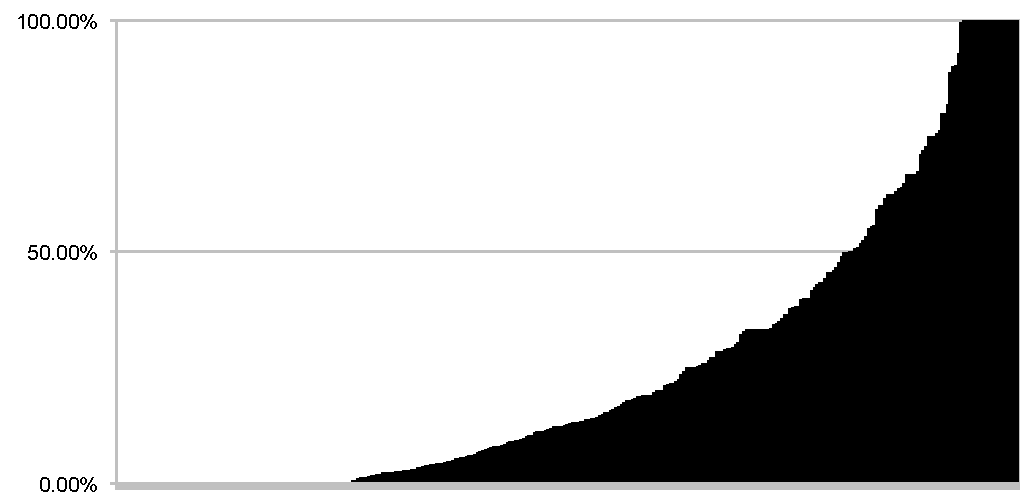
\includegraphics[width=\columnwidth]{images/percentage_elimination}
\end{center}
\caption{\label{fig:percentage_elimination}
Percentage of overflow checks that our range analysis removes.
Each bar is a benchmark in the LLVM test suite.
Benchmarks have been ordered by the effectiveness of the range analysis.
On average, we have eliminated 24.93\% of the checks (geomean).}
\end{figure}

Figure~\ref{fig:spec_runtime} shows the impact of our instrumentation in the
runtime of the SPEC benchmarks.
We ran each benchmark 20 times.
The largest slowdown that we have observed, 11.83\%, happened in
\texttt{h264ref}, the benchmark that presented the largest number of distinct
sites where overflows happened dynamically. 
On the average, the instrumented programs are 3.24\% slower than the
original benchmarks.
If we use the range analysis to eliminate overflow checks, this slowdown falls
to 1.73\%.
The range analysis, in this case, reduces the instrumentation overhead by
46.60\%.
This improvement is larger than the percentage of overflow checks that we
avoid, e.g,. 20.57\%.
We believe that this difference is due to the fact that we are able to
eliminate checks on induction variables, as our range analysis can rely on
the loop boundaries to achieve this end.
We have not noticed any runtime difference between programs converted to
e-SSA form or u-SSA form.
Surprisingly, some of the instrumented programs run faster than the original
code.
This behavior has also been observed by Dietz {\em et al.}~\cite{Dietz12}.

\begin{figure}[t!]
\begin{center}
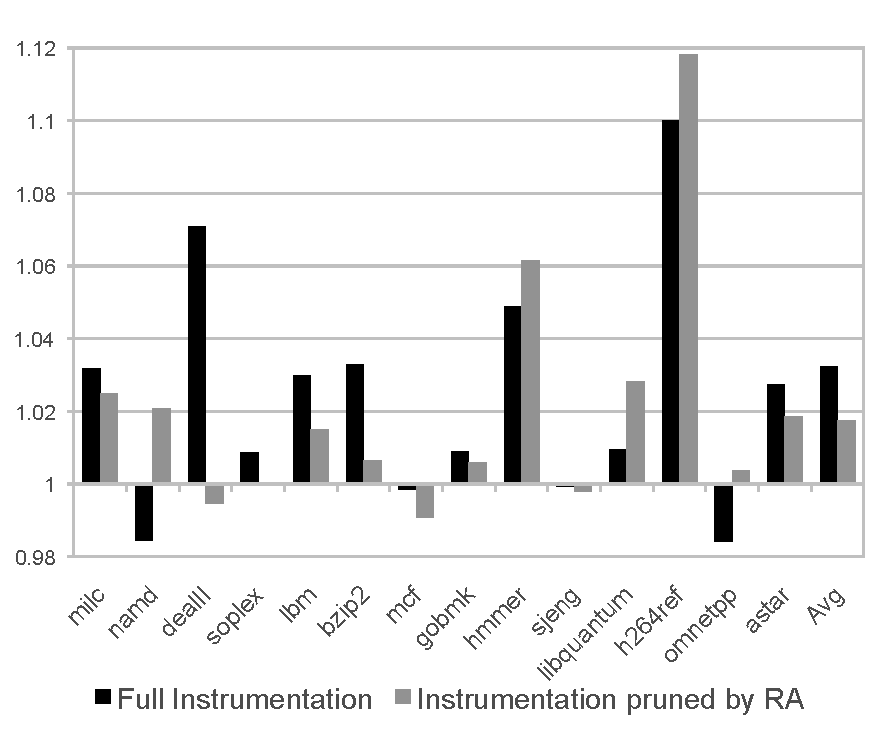
\includegraphics[width=\columnwidth]{images/spec_runtime}
\end{center}
\caption{\label{fig:spec_runtime}
Comparison between execution times with and without pruning, 
normalized by the original program's execution time.}
\end{figure}


\section{Related Work}
\label{sec:rel}

\noindent
\textbf{Dynamic Detection of Integer Overflows: }
Brumley {\em et al.}~\cite{Brumley07} have developed a tool, RICH, to
secure C programs against integer overflows.
The author's approach consists in instrumenting every integer operation that
might cause an overflow, underflow, or data loss.
The main result of Brumley {\em et al.} is the verification that guarding programs
against integer overflows does not compromise their
performance significantly: the average slowdown across four large applications
is 5\%.
RICH, Brumley {\em et al}'s tool, uses specific features of the x86 architecture
to reduce the instrumentation overhead.
Chinchani {\em et al.}~\cite{Chinchani04} follow a similar approach.
In this work, the authors describe each arithmetic operation formally, and then
use characteristics of the computer architecture to detect overflows at
runtime.
% TODO bibtex: cite Archerr: Runtime environment driven program safety.
Contrary to these previous works, we instrument programs at LLVM's intermediate
representation level, which is machine independent.
Nevertheless, the performance of the programs that we instrument is on par with
Brumley's, even without the support of the static range analysis.
Furthermore, our range analysis could eliminate approximately
45\% of the tests that a naive implementation of Brumley's technique
would insert; hence, halving down the runtime overhead of instrumentation.

Dietz {\em et al.}~\cite{Dietz12} have 
implemented a tool, IOC, that instruments the source code of C/C++ programs to
detect integer overflows.
They approach the problem of detecting integer overflows from a software
engineering point-of-view; hence, performance is not a concern.
The authors have used IOC to carry out a study about the occurrences
of overflows in real-world programs, and have found that these events are very
common.
It is possible to implement a dynamic analysis without instrumenting the
target program.
In this case, developers must use some form of code emulation.
Chen {\em et al.}~\cite{Chen09}, for instance, uses a modified
Valgrind~\cite{Nethercote07} virtual machine to detect integer overflows.
The main drawback of emulation is performance: Chen {\em et al.} report a
50x slowdown.
% TODO: cite "Brick: A  binary tool for run-time detecting and locating
% integer-based vulnerability.
We differ from all this previous work because we focus on generating less
instrumentation, an endeavor that we accomplish via static analysis.

\noindent
\textbf{Static Detection of Integer Overflows: }
Zhang {\em et al.}~\cite{Zhang10} have used static analysis to sanitize
programs against integer overflow based vulnerabilities.
They instrument integer operations in paths from a source to a sink.
In Zhang {\em et al.}'s context, sources are functions that read values from
users, and sinks are memory allocation operations.
Thus, contrary to our work, Zhang {\em et al.}'s only need to instrument
about 10\% of the integer operations in the program.
However, they do not use any form of range analysis to limit the number of
checks inserted in the transformed code.
Wang {\em et al.}~\cite{Wang09} have implemented a tool, IntScope, that combines symbolic execution and taint analysis to detect integer overflow vulnerabilities. The authors have been able to use this tool to successfully identify many vulnerabilities in industrial quality software. Our work, and Wang {\em et a.}'s work are essentially different: they use symbolic execution, whereas we rely on
range analysis.
Contrary to us, they do not transform the program to prevent or detect such event dynamically.
Still in the field of symbolic execution, Molnar
{\em et al.}~\cite{Molnar09} have implemented a tool, SmartFuzz, that analyzes
Linux x86 binaries to find integer overflow bugs.
They prove the existence of bugs by generating test cases for them.

\noindent
\textbf{Range Analysis and sparse representations:}
One of the goals of this paper is to describe a state-of-the-art range analysis
algorithm.
Many parts of this algorithm are well-known, others are novel.
The widening and narrowing operators from Section~\ref{sub:micro} were
introduced by Cousot and Cousot's seminal paper~\cite{Cousot77}.
The widening operator that we use in our implementation is well-known among
compiler writers~\cite[p.228]{Nielson99}.
The interval lattice from Section~\ref{sub:lattice} has been used in a
plethora of old and recent range analysis
solvers~\cite{Gough94,Gawlitza09,Logozzo10,Mahlke01,Oh12,Patterson95,Stephenson00,Su05}.
The use of futures to handle comparisons between variables is a contribution
of this paper.
It is well-known that the use of strongly connected components speeds up
constraint resolution systems~\cite[Sec 6.3]{Nielson99}.
However, publicly available implementations of range analysis such as those in
FLEX~\footnote{The MIT's FLEX/Harpoon compiler
provides an implementation of Stephenson's algorithm~\cite{Stephenson00}, and
is available at \texttt{http://flex.cscott. net/Harpoon/}.},
gcc~\footnote{Gcc's VRP pass (at \texttt{http://gcc.gnu.org/svn/gcc/trunk/gcc/
tree-vrp.c}) implements a variant of Patterson's
algorithm~\cite{Patterson95}.} or Mozilla's IonMonkey~\footnote{\texttt{hg.mozilla.org/projects/ionmonkey/file/629d1e6251b9/js/
src/ion/RangeAnalysis.cpp}. This code is implemented after Gough and
Klaeren~\cite{Gough94}} do not resort to this technique.
Furthermore, they only deal with comparisons between variables and constants.
The only work that we are aware of that has used range analysis to avoid
overflow checks is Sol {\em et al}'s~\cite{Sol11}; however, their algorithm
is much more limited than ours.
Contrary to us, Sol {\em et al.} eliminate overflow checks in
straight-line code traces produced by a just-in-time compiler, and they use the
runtime values of variables to improve their precision.


In this paper we provide a {\em sparse} implementation of range analysis.
Sparsity, in our context, means that we associate points in the lattice of
interest -- intervals in our case -- directly to variables.
Dense analyses map such information to pairs formed by variables and program
points.
Some previous analyses have achieved sparsity by using specific program
representations, like we did.
One of the program representations that we discuss in
Section~\ref{sub:splitting} -- the {\em
Extended Static Single Assignment} (e-SSA) form -- has been used by Bodik
{\em et al.}~\cite{Bodik00} and Gough {\em et al.}~\cite{Gough94}.
The other representation, which we call u-SSA, is very similar to
the \emph{Static Single Use} form (SSU).
There exist other variants of SSU~\cite{Lo98,Plevyak96,George03}.
The main difference to our representation is that our dataflow analysis
propagates information forwardly, whereas the SSU form has been conceived for
dataflow analyses that propagate information backwardly.
Thus, it requires special nodes at branches to merge information from
different program paths.
The SSU form programs are a subset of the programs in the so called
{\em Static Single Information} form, a program representation proposed by
Scott Ananian~\cite{Ananian99}.
SSI makes sparse the dataflow analyses that propagate information both
forwardly and backwardly.

\section{Final Remarks}
\label{sec:rem}

This paper has presented a static range analysis algorithm that reduces
the overhead necessary to secure programs against integer overflows.
This algorithm analyzes inter-procedurally programs with
half-a-million lines of code, i.e., almost one million constraints, in
ten seconds.
We proposed the notion of ``future bounds" to handle comparisons
between variables, and tested different program representations to improve our
precision.
Although the overhead of guarding programs against integer overflows is small,
as previous work has demonstrated, we believe that our technique is still
important, as some of these programs will be executed millions of times.
Our entire code plus the data that we show in this paper is publicly available.
A more extensive list of experiments is also available in our technical report.

\acks
We thank Douglas do Couto and Igor Costa for helping us with the LLVM code
base.
We also thank the anonymous reviewers for their useful comments and
suggestions.
This project is supported by FAPEMIG, grant 16899*01.

\bibliographystyle{plain}
\bibliography{../references}

\end{document}
